% !TeX spellcheck = french
\documentclass[a4paper,french,final]{memoir}
\usepackage{luacode}
\usepackage[german,main=french]{babel}
\usepackage[autostyle=true,maxlevel=3]{csquotes}
\usepackage{microtype}
\usepackage{fontspec}
\usepackage{geometry}
\usepackage{mathtools} 
\usepackage[math-style=french,warnings-off={mathtools-colon,mathtools-overbracket}]{unicode-math}
\setmainfont{TeX Gyre Termes}
\setmathfont{TeX Gyre Termes Math}
\setmathfont[range=bb]{STIX Two Math}
\setmathfont[range={scr,cal}]{TeX Gyre Pagella Math}
\usepackage[amsmath,thmmarks,hyperref]{ntheorem}
\usepackage[most]{tcolorbox}
\usepackage{xparse,xpatch}
\usepackage{tikz}
\usepackage{caption}
\usetikzlibrary{calc,trees,positioning,arrows,fit,shapes,calc}
\usepackage{lualatex-math}
\usepackage[unicode,naturalnames]{hyperref}
\usepackage{cleveref}
\AtBeginDocument{\let\savedemptyset\emptyset} % 
\AtBeginDocument{\let\emptyset\varnothing} % 
\AtBeginDocument{\let\savedleq\leq} % 
\AtBeginDocument{\let\savedgeq\geq} %
\AtBeginDocument{\let\leq\leqslant} % 
\AtBeginDocument{\let\geq\geqslant} %
\newcommand{\paral}{\mathrel{\!/\mkern-5mu/\!}} % \parallel existe déjà : || vs //
\makeatletter
\newcommand*{\theauthor}{\@author}
\newcommand*{\thetitle}{\@title}
\newcommand*{\thedate}{\@date}
\renewcommand{\xmapsto}[2][]{\mathrel{\mathpalette\xmapsto@{{#1}{#2}}}}
\renewcommand{\xmapsto}[2][]{\mathrel{\mathpalette\xmapsto@{{#1}{#2}}}}
\newcommand{\xmapsto@}[2]{\xmapsto@@{#1}#2}
\newcommand{\xmapsto@@}[3]{%
  \begingroup
  \sbox\z@{$\m@th#1\mathop{}\limits_{\;#2\;}^{\;#3\;}$}%
  \mathop{\Uhextensible width \wd\z@ 0 "27FC}_{#2}^{#3}%
  \endgroup
}
\renewcommand{\xLeftrightarrow}[2][]{\mathrel{\mathpalette\xLeftrightarrow@{{#1}{#2}}}}
\newcommand{\xLeftrightarrow@}[2]{\xLeftrightarrow@@{#1}#2}
\newcommand{\xLeftrightarrow@@}[3]{%
  \begingroup
  \sbox\z@{$\m@th#1\mathop{}\limits_{\;#2\;}^{\;#3\;}$}%
  \mathop{\Uhextensible width \wd\z@ 0 "027FA}_{#2}^{#3}% 027FA code for long left right double arrow in unicode-math-table.tex 
  \endgroup
}

\newcounter{proofpart}
\newcommand{\proofpart}{\@ifstar{\@proofpart}{\@@proofpart}}

\newcommand{\@proofpart}[1]{%
  \if\detokenize{#1}\relax\else{
  \par
  \addvspace{\medskipamount}%
  \noindent \itshape%
  {#1~:\par\nobreak\smallskip}%
  \normalfont
  \@afterheading
}\fi
}

\newcommand{\@@proofpart}[1]{%
  \par
  \addvspace{\medskipamount}%
  \stepcounter{proofpart}%
  \noindent Partie \theproofpart~:~\itshape%
  \if\detokenize{#1}\relax%
  \else{#1.}\fi%
  \par\nobreak\smallskip
  \normalfont
  \@afterheading
}
\makeatother
%%%%%%%%%%%%%%%%%%%%%%%%%%%%%%%%%%%%%%%%%%%%%%%%
%            NUMEROTATION (CLASSE MEMOIR)       %
%%%%%%%%%%%%%%%%%%%%%%%%%%%%%%%%%%%%%%%%%%%%%%%%%
\setsecnumdepth{subsubsection}
\renewcommand{\cftpartaftersnum}{.}
\renewcommand{\cftchapteraftersnum}{.}
\renewcommand{\cftpartdotsep}{\cftdotsep}
\renewcommand{\cftchapterdotsep}{\cftdotsep}% Chapters should use dots in ToC
\aliaspagestyle{title}{empty} 
\aliaspagestyle{part}{empty} 
%\setlength\headheight{\dimexpr \headheight+0.20004pt}

\usepackage[backend=biber,style=alphabetic]{biblatex}
\addbibresource{references.bib}
%%%%%%%%%%%%%%%%%%%%%%%%%%%%%
%   THEOREMES SANS BOITES   %
%%%%%%%%%%%%%%%%%%%%%%%%%%%%%
\theoremstyle{break}
\theoremseparator{~:} % espace fine insécable avant le :
\newtheorem{lemma}{Lemme}
\newtheorem{corollary}{Corollaire}
\newtheorem{definition}{Définition}
\theoremstyle{plain}
\newtheorem*{question}{Question}
\newtheorem*{answer}{Réponse}
\newtheorem{remark}{Remarque}
\theoremsymbol{\text{\bsc{c.q.f.d}}} % mod
\theorembodyfont{\normalfont}
\theoremprework{\setcounter{proofpart}{0}}
\newtheorem*{proof}{Démonstration}
%%%%%%%%%%%%%%%%%%%%%%%%%%%%%
%            COULEURS       %
%%%%%%%%%%%%%%%%%%%%%%%%%%%%%
\definecolor{vert}{RGB}{0,181,0}
\definecolor{oran}{RGB}{223,74,0}
\definecolor{viol}{RGB}{134,0,175}
\definecolor{roug}{RGB}{215,15,0}
\definecolor{bleu}{RGB}{0,104,180}

%%%%%%%%%%%%%%%%%%%%%%%%%%%%%
%   BOITES POUR THEOREMES   %
%%%%%%%%%%%%%%%%%%%%%%%%%%%%%
\tcbset{separator sign={},
        description delimiters parenthesis,
        label separator=-,
styletheorem/.style={enhanced,
  coltitle=black,
  colback=white,
  fonttitle=\bfseries,
  boxrule=\fboxrule,
  boxed title style={boxrule=\fboxrule},
  attach boxed title to top left={yshift=-2mm, xshift=2mm},
    }%
}
\newtcbtheorem[auto counter, number within = section]
{theoremb}{Théorème}{styletheorem,colframe=roug,
colback=white!90!roug,colbacktitle=white!80!roug,label type=theorem}{thm}
\newtcbtheorem[auto counter, number within = section]
{remarkb}{Remarque}{styletheorem,colframe=oran,
colbacktitle=white!80!oran,colback=white!90!oran,label type=remark}{rem}
\newtcbtheorem[auto counter, number within = section]
{defb}{Définition}{styletheorem,colframe=bleu,
colbacktitle=white!80!bleu,colback=white!90!bleu,label type=definition}{def}
\newtcbtheorem[auto counter, number within = section]
{noteb}{Commentaire}{styletheorem,colframe=vert,
colbacktitle=white!80!vert,colback=white!90!vert,label type=note}{note}
% le label type fait automatiquement la jonction avec cleveref pour nommer les théorèmes : le dernier groupe (thm,rem,def) permet de créer des labels automatiquement. 

%%%%%%%%%%%%%%%%%%%%%%%%%%%%%%%%%%
%  SEPARATEUR (DANS LES PREUVES) : \proofpart   %
%%%%%%%%%%%%%%%%%%%%%%%%%%%%%%%%%%%
% une  commande est définie pour séparer les preuves en deux variantes : avec et sans étoiles. (\proofpart et \proofpart*)
% Par défaut, elle crée des sous parties dans un environement de démonstration sous la forme 
% " Partie n : [titre en italique]. ", où n est un entier naturel strictement positif. Dans le cas ou le titre est vide, le point (.) n'est pas ajouté. Si le titre est vide, il faut utiliser \proofpart{}
% Avec une étoile, on obtient 
%[titre en italique : ] 

\newcommand{\deffunct}[5]{%
\begin{align*}%
      #1 \colon & #2 \to #3\\
       &#4\xmapsto{\hphantom{#1}} #5
\end{align*}%
}
%%%%%%%%%%%%%%%%%%%%%%%%%%%%%
%   PAGE DE GARDE            %
%%%%%%%%%%%%%%%%%%%%%%%%%%%%%
\newcommand{\HRule}{\rule{\paperwidth}{0.5mm}} % trait, régler eppaisseur
\newcommand*{\theuniversity}{Université de Toulon}
\newcommand*{\theyearname}{Licence de Mathématiques, parcours mathématiques, 
2\ieme~année}
\newcommand*{\thesupervisor}{Joachim \bsc{Asch}}
\author{Anastasiia \bsc{Chernetcova}~\&~Tom \bsc{Domenge}}
\title{Projet TER 2020\par
            Dénombrabilité : \par $\mathbb{N},2\mathbb{N} \ \& \ \mathbb{Q}$\par}

%%%%%%%%%%%%%%%%%%%%%%%%%%%%%%%%%%%%%%%%%%%%%%
%   Opérateurs (dans le style de max etc.   %
%%%%%%%%%%%%%%%%%%%%%%%%%%%%%%%%%%%%%%%%%%%%%%
\DeclareMathOperator{\Card}{Card} % s'utilise avec \Card en mode maths
\makeatletter
\newcommand{\diagdenomb}{\@ifstar{\@diagdenomb}{\@@diagdenomb}}
\newcommand{\@diagdenomb}{\begin{figure}[htbp]
    \centering
\begin{tikzpicture}
\tikzstyle{keepstyle} =[rectangle, rounded corners, draw, fill=white]
\node at (0,0) {$\vdots$};
\node[keepstyle] (51) at (0,1) {$\frac{5}{1}$};
\node[keepstyle] (41) at (0,2) {$\frac{4}{1}$};
\node[keepstyle] (31) at (0,3) {$\frac{3}{1}$};
\node[keepstyle] (21) at (0,4) {$\frac{2}{1}$};
\node[keepstyle] (11) at (0,5) {$\frac{1}{1}$};
\node at (1,0) {$\vdots$};
\node[keepstyle] (52) at (1,1) {$\frac{5}{2}$};
\node at (1,2) {$\frac{4}{2}$};
\node[keepstyle] (32) at (1,3) {$\frac{3}{2}$};
\node at (1,4) {$\frac{2}{2}$};
\node[keepstyle] (12) at (1,5) {$\frac{1}{2}$};
\node at (2,0) {$\vdots$};
\node at (2,1) {$\frac{5}{3}$};
\node[keepstyle] (43) at (2,2) {$\frac{4}{3}$};
\node at (2,3) {$\frac{3}{3}$};
\node[keepstyle] (23) at (2,4) {$\frac{2}{3}$};
\node[keepstyle] (13) at (2,5) {$\frac{1}{3}$};
\node at (3,0) {$\vdots$};
\node at (3,1) {$\frac{5}{4}$};
\node at (3,2) {$\frac{4}{4}$};
\node[keepstyle] (34) at (3,3) {$\frac{3}{4}$};
\node at (3,4) {$\frac{2}{4}$};
\node[keepstyle] (14) at (3,5) {$\frac{1}{4}$};
\node at (4,0) {$\vdots$};
\node  at (4,1) {$\frac{5}{5}$};
\node at (4,2) {$\frac{4}{5}$};
\node at (4,3) {$\frac{3}{5}$};
\node[keepstyle] (25) at (4,4) {$\frac{2}{5}$};
\node[keepstyle] (15) at (4,5) {$\frac{1}{5}$};
\node at (5,0) {$\vdots$};
\node  at (5,1) {$\frac{5}{6}$};
\node at (5,2) {$\frac{4}{6}$};
\node at (5,3) {$\frac{3}{6}$};
\node at (5,4) {$\frac{2}{6}$};
\node[keepstyle] (16) at (5,5) {$\frac{1}{6}$};
\node at (6,1) {$\cdots$};
\node at (6,2) {$\cdots$};
\node at (6,3) {$\cdots$};
\node at (6,4) {$\cdots$};
\node at (6,5) {$\cdots$};
\draw [-latex,red, thick] (11) -- (12);
\draw [-latex, red, thick] (12) -- (21);
\draw [-latex, red, thick] (21) -- (31);
\draw [-latex, red, thick] (31) -- (13);
\draw [-latex, red, thick] (13) -- (14);
\draw [-latex, red, thick] (14) -- (23);
\draw [-latex, red, thick] (23) -- (32);
\draw [-latex, red, thick] (32) -- (41);    
\draw [-latex, red, thick] (41) -- (51);
\draw [-latex, red, thick] (51) -- (15);
\draw [-latex, red, thick] (15) -- (16);
\draw [-latex, red, thick] (16) -- (25);
\draw [-latex, red, thick] (25) -- (34);
\draw [-latex, red, thick] (34) -- (43);
\draw [-latex, red, thick] (43) -- (52);
\end{tikzpicture}
%\caption*{Dénombrabilité de $\mathbb{Q}$}
\end{figure}
}
\newcommand{\@@diagdenomb}{\begin{figure}[htbp]
    \centering
\begin{tikzpicture}
\tikzstyle{keepstyle} =[rectangle, rounded corners, draw, fill=white]
\node at (0,0) {$\vdots$};
\node[keepstyle] (51) at (0,1) {$\frac{5}{1}$};
\node[keepstyle] (41) at (0,2) {$\frac{4}{1}$};
\node[keepstyle] (31) at (0,3) {$\frac{3}{1}$};
\node[keepstyle] (21) at (0,4) {$\frac{2}{1}$};
\node[keepstyle] (11) at (0,5) {$\frac{1}{1}$};
\node at (1,0) {$\vdots$};
\node[keepstyle] (52) at (1,1) {$\frac{5}{2}$};
\node at (1,2) {$\frac{4}{2}$};
\node[keepstyle] (32) at (1,3) {$\frac{3}{2}$};
\node at (1,4) {$\frac{2}{2}$};
\node[keepstyle] (12) at (1,5) {$\frac{1}{2}$};
\node at (2,0) {$\vdots$};
\node at (2,1) {$\frac{5}{3}$};
\node[keepstyle] (43) at (2,2) {$\frac{4}{3}$};
\node at (2,3) {$\frac{3}{3}$};
\node[keepstyle] (23) at (2,4) {$\frac{2}{3}$};
\node[keepstyle] (13) at (2,5) {$\frac{1}{3}$};
\node at (3,0) {$\vdots$};
\node at (3,1) {$\frac{5}{4}$};
\node at (3,2) {$\frac{4}{4}$};
\node[keepstyle] (34) at (3,3) {$\frac{3}{4}$};
\node at (3,4) {$\frac{2}{4}$};
\node[keepstyle] (14) at (3,5) {$\frac{1}{4}$};
\node at (4,0) {$\vdots$};
\node  at (4,1) {$\frac{5}{5}$};
\node at (4,2) {$\frac{4}{5}$};
\node at (4,3) {$\frac{3}{5}$};
\node[keepstyle] (25) at (4,4) {$\frac{2}{5}$};
\node[keepstyle] (15) at (4,5) {$\frac{1}{5}$};
\node at (5,0) {$\vdots$};
\node  at (5,1) {$\frac{5}{6}$};
\node at (5,2) {$\frac{4}{6}$};
\node at (5,3) {$\frac{3}{6}$};
\node at (5,4) {$\frac{2}{6}$};
\node[keepstyle] (16) at (5,5) {$\frac{1}{6}$};
\node at (6,1) {$\cdots$};
\node at (6,2) {$\cdots$};
\node at (6,3) {$\cdots$};
\node at (6,4) {$\cdots$};
\node at (6,5) {$\cdots$};
\draw [-latex,red, thick] (11) -- (12);
\draw [-latex, red, thick] (12) -- (21);
\draw [-latex, red, thick] (21) -- (31);
\draw [-latex, red, thick] (31) -- (13);
\draw [-latex, red, thick] (13) -- (14);
\draw [-latex, red, thick] (14) -- (23);
\draw [-latex, red, thick] (23) -- (32);
\draw [-latex, red, thick] (32) -- (41);    
\draw [-latex, red, thick] (41) -- (51);
\draw [-latex, red, thick] (51) -- (15);
\draw [-latex, red, thick] (15) -- (16);
\draw [-latex, red, thick] (16) -- (25);
\draw [-latex, red, thick] (25) -- (34);
\draw [-latex, red, thick] (34) -- (43);
\draw [-latex, red, thick] (43) -- (52);
\end{tikzpicture}
\caption{Dénombrabilité de $\mathbb{Q}$}
    \label{fig-denombQ}
\end{figure}
}
\makeatother
\graphicspath{{./figures/}} % pour les images, plus besoin d'écrire "./figures"
\newcommand{\diagbij}{\begin{figure}[htbp]
	\centering
	\begin{tikzpicture}[ele/.style={fill=black,circle,minimum width=.8pt,inner sep=1pt},every fit/.style={ellipse,draw,inner sep=-2pt}]
	\node[ele,label=left:$a$] (a1) at (0,4) {};    
	\node[ele,label=left:$b$] (a2) at (0,3) {};    
	\node[ele,label=left:$c$] (a3) at (0,2) {};
	\node[ele,label=left:$d$] (a4) at (0,1) {};
	\node[ele,label=left:$d$] (a5) at (0,1) {};
	\node[ele,fill=roug,label=right:$1$] (b1) at (4,4) {};
	\node[ele,fill=roug,label=right:$2$] (b2) at (4,3) {};
	\node[ele,fill=roug,label=right:$3$] (b3) at (4,2) {};
	\node[ele,fill=roug,label=right:$4$] (b4) at (4,1) {};
	
	\node[fill=bleu,draw=bleu,fill opacity=0.3,fit= (a1) (a2) (a3) (a4) (a5),minimum width=2cm] {} ;
	\node[fill=roug,draw=roug,fill opacity=0.3,fit= (b1) (b2) (b3) (b4),minimum width=2cm] {} ;  
	\draw[->,thick,shorten <=2pt,shorten >=2] (a1) -- (b4);
	\draw[->,thick,shorten <=2pt,shorten >=2] (a2) -- (b2);
	\draw[->,thick,shorten <=2pt,shorten >=2] (a3) -- (b1);
	\draw[->,thick,shorten <=2pt,shorten >=2] (a4) -- (b3);
	\end{tikzpicture}
	\caption{diagramme d'une fonction bjective}
	\label{fig-fonctbij}
\end{figure}}
\begin{document}
\begin{titlingpage}
\setlrmargins{*}{*}{1}
\checkandfixthelayout[nearest] 
\vspace*{\fill}%
\begin{center}
\vspace*{\fill}%
\makebox[\linewidth]{\HRule} % demande à latex l'espace pour le trait
\parbox[t]{\textwidth}{\addvspace{\parskip} % on ajoute ce qu'il faut d'espace pour sous le trait
\centering\huge\bfseries\thetitle}
 \null%Espace obligatoire pour LaTeX (boite vide) sinon l'espace est ignoré
\vspace*{\parskip}
\makebox[\linewidth]{\HRule}
\vspace*{\fill}
\diagdenomb*
\vspace{\fill}
\par \Large Rédigé par \theauthor\par Supervisé par \thesupervisor \par
\vspace*{\fill}
\large{\theyearname.\par \theuniversity, Version du \thedate}
\end{center}

\end{titlingpage}
\frontmatter
\tableofcontents
\part{Introduction}

\chapter{Avant-propos}

La notion de l'infini (noté $\infty$) apparaît pour la première fois lorsqu'on étudie l'ensemble des entiers naturels. C'est une définition intuitive de l'infini. L'infini n'est pas un nombre, il n'obéit pas aux lois usuelles $+$ et $\times$ de la même manière que les nombres réels. En mathématiques, l'une des manières les plus simples de caractériser l'infini est celle de la théorie des ensembles. L'une des propriétés principales d'un ensemble est sa taille. Comme nous allons le voir, les ensembles mathématiques peuvent être finis ou infinis.

L'étude des ensembles infinis est révélatrice de paradoxes, l'un des plus célèbres  énonce qu'une partie stricte d'un ensemble infini peut contenir autant d'éléments que l'ensemble lui-même. C'est le paradoxe de l'hôtel de \bsc{Hilbert} (1924).

On peut alors se poser des questions fondamentales à l'étude de l'infini : comment peut on caractériser les ensembles infinis ? Est-ce qu'il y a un infini << plus grand >> ou << plus petit >> que celui des nombres ?  

Dans la première partie, nous allons rappeler ce que sont les ensembles, cruciaux pour l'étude de l'infini du point de vuel' ensembliste, et introduire une axiomatique de $\mathbb{N}$. Dans la seconde partie, nous nous consacrerons à l'étude de dénombrabilité d'ensembles usuels et aux propriétés d'ensembles dénombrables.\\

\epigraph{%
	\enquote{\itshape Der Mathematiker abstrahiert gänzlich von der Beschaffenheit der Gegenstände und dem Inhalt ihrer Relationen; er hat es bloß mit der Abzählung und Vergleichung der Relationen unter sich zu tun.}\newline \newline
\enquote{Le mathématicien fait fi de la nature des objets qu'il manipule, et des relations qu'ils entretiennent ; il lui suffit de les passer en revue et de les comparer entre elles.}
}{Carl Friedrich \bsc{Gauss}\footnotemark}\footcitetext{gauss_cite}
\chapter{Notations}
\mainmatter
<<<<<<< HEAD
\part{Préliminaires au dénombrement}
=======
\part{Préliminaires au dénombrement : Notion de comptage}
\chapter{\texorpdfstring{Définition de $\mathbb{N}$}{Définition de N}}
aa
>>>>>>> b9f082087e06fb175367072ac3aaa6c8e944d51d
\chapter{Rappels de théorie des ensembles}

\chapter{Définition de la cardinalité}
\part{Dénombrabilité}
\chapter{Définition et propriétés de la dénombrabilité}

\section{Ensembles finis et infinis}

\begin{defb}{Finitude}{fini}
     Soit $E$ un ensemble. 
	    
	On dit que $E$ est fini si $E = \emptyset$ ou s'il existe une bijection $\varphi : \{1,\dots,n \} \to E$, avec $n \in \mathbb{N}$. 
		
	Dans ce cas, on dit que $E$ est de cardinal $n$ (ou de puissance $n$), et on note le cardinal $\Card(E)$. 
\end{defb}

\begin{defb}{Equipotence}{equip}
    On dit que $E$ et $F$ sont équipotents ssi $\Card(E) = \Card(F)$ s' il existe $\varphi : E \to F$ bijective. Dans ce cas, on note $E \mathrel{\approx} F$. 
\end{defb}

\begin{theoremb}{}{mmpuiss}
    $ \mathrel{\approx}$ est une relation d'équivalence. 
\end{theoremb}

\begin{proof}
    Soient $E, F, G$ 3 ensembles finis.
	\begin{enumerate} 
		\item $E \mathrel{\approx} E$ étant donné que $E$ a le même cardinal que E. $\mathrel{\approx}$ est réflexive.
		\item $E \mathrel{\approx} F$ signifie que $ \Card(E) = \Card(F)$ et par symétrie de l'égalité, $\Card(F) = \Card(E)$, ie $F \mathrel{\approx} E$. $\mathrel{\approx}$ est symétrique. 
		\item Si $E \mathrel{\approx} F$ et $F \mathrel{\approx} G$ alors $\Card(E) = \Card(F)$ et $\Card(F) = \Card(G)$. Par transitivité de l'égalité, $\Card(E) = \Card(G)$, ie $E \mathrel{\approx} G$. $\mathrel{\approx}$ est transitive. 
	\end{enumerate}
	$\mathrel{\approx}$ est bien une relation d'équivalence.
\end{proof}

\begin{theoremb}{}{assequiv}
	Soient $E, F$ deux ensembles et $\varphi : E \to F$ une application. Si $E \mathrel{\approx} F$ alors les 3 assertions suivantes sont équivalentes :
	
	\begin{enumerate}
		\item $\varphi$ est injective ;
		\item $\varphi$ est surjective ;
		\item $\varphi$ est bijective. 
	\end{enumerate}
\end{theoremb}

\begin{defb}{Ensemble infini}{ifini}
	Soit $E$ un ensemble.
	
	On dit que $E$ est infini ssi $E$ n'est pas fini.
\end{defb}

\begin{theoremb}{}{partn} 
	Toute partie de $\mathbb{N}$ est finie ssi elle est majorée. 
\end{theoremb}



\begin{theoremb}{}{ninfini}
	$\mathbb{N}$ est infini. 
\end{theoremb}


\begin{proof}
	Si $\mathbb{N}$ était fini, d'après le \cref{thm-partn}, $\mathbb{N}$ admettrait un majorant. Autrement dit \[\exists k \in \mathbb{N}, \forall x \in \mathbb{N}, x \leq k.\]

	Or la construction de $\mathbb{N}$ implique que si $ k \in \mathbb{N}$, alors $k + 1 \in \mathbb{N}$ et $\exists x \in \mathbb{N}, x > k, x= k+1$, d'où une contradiction. 
	
	Donc $\mathbb{N}$ est infini.
\end{proof}

\section{Ensembles dénombrables}

\begin{defb}{Ensemble démombrable, au plus dénombrable}{denomb}

	 Soit $E$ un ensemble infini. 
	 
	 On dit que $E$ est dénombrable ssi il existe une application $\varphi : \mathbb{N} \to E $ bijective. 
	 
	 Un ensemble fini ou dénombrable est dit au plus dénombrable. 
\end{defb}

On note par la suite $\aleph_0$, lire \emph{aleph zéro,} la puissance de $\mathbb{N}$. 

\begin{proof}
a
\proofpart{test}
soit
\end{proof}

\chapter{Propriétés usuelles de dénombrabilité}

\begin{theoremb}{}{parties}

	Soient $E$ et $F$ deux ensembles. 
	Si $E \subset F$ et si $F$ est dénombrable, alors $E$ est au plus dénombrable.
\end{theoremb}

\begin{theoremb}{Union de deux ensembles dénombrables}{union}
    Soit $(A_i)_{i \in I}$ une famille dénombrable. 
	
	Alors $A= \bigcup_{i \in I} A_i$ est dénombrable. 
\end{theoremb}


\begin{theoremb}{Produit cartésien d'ensembles dénombrables}{cartesien}
	Soient $A, B, A_1, \dots, A_i, \dots, A_n$ des ensembles dénombrables. 
	
	\begin{enumerate}
		\item Le produit cartésien $A \times B$ est dénombrable. 
		\item Plus généralement, tout produit \textbf{fini} $\prod_{i=1}^{n} A_i $ est dénombrable.
	\end{enumerate}
\end{theoremb}

\begin{proof}
	Les  \cref{thm-union,thm-cartesien} seront démontrées par la suite dans la \cref{sec-denombrabilite_usuelle}~.
	
	% saut de ligne pour virer le cqfd
\end{proof}




\chapter{\texorpdfstring{Dénombrabilité de 2$\mathbb{N}$, $\mathbb{Z}$, $\mathbb{Q}$}{Dénombrabilité de Q}} 
\section{ \texorpdfstring{Dénombrabilité de 2$\mathbb{N}$}{}}
\label{sec-denombrabilite_usuelle}
Naturellement on pourrait penser que les ensembles inclus dans $\mathbb{N}$ ont une puissance inférieure à $\aleph_0$. Contre toute attente, voici un résultat sur la dénombrabilité de  $2\mathbb{N}$, l'ensemble des entiers naturels pairs.

\begin{theoremb}{Dénombrabilité de 2$\mathbb{N}$}{}
	L'ensemble 2$\mathbb{N}$ des entiers naturels pairs est dénombrable. 
\end{theoremb}

\begin{proof}
	On construit l'application \[ \begin{array}{cccc}
	\ & \mathbb{N}& \to& 2\mathbb{N} \\
	\varphi : & n & \mapsto & 2n
	\end{array}.\]
	
	Cette application $\varphi $ est bijective car sa réciproque est $ \varphi^{-1} : \begin{array}{ccc}
	2\mathbb{N} & \to & \mathbb{N}\\
	k & \mapsto & \frac{k}{2}
	\end{array}$. 
	
	2$\mathbb{N}$ est en bijection avec $\mathbb{N}$. 2$\mathbb{N}$ est bien un ensemble dénombrable de puissance $\aleph_0$. 
\end{proof}

On peut introduire un résultat plus général qui couvre toute partie de $\mathbb{N}$. 

\begin{theoremb}{Dénombrabilité des parties infinies de $\mathbb{N}$}{}
	Toute partie $E \subset \mathbb{N}$ infinie a le même cardinal que $\mathbb{N}$. 
\end{theoremb}

\begin{proof}
	On construit, par récurrence, une bijection $\phi : \mathbb{N} \to E$ telle que: 
	
	\[\left\lbrace \begin{array}{c}
	\phi(0) = \min \{x \in E\} \\
	\forall n \in \mathbb{N}, \phi(n+1) = \min \{x \in E, x > \phi(n) \}
	\end{array} \right.\]
	
	C'est bien une bijection : elle est injective et surjective car $\forall k \in \mathbb{N}, k \leq \phi(k)$. 
\end{proof}

\section{\texorpdfstring{Dénombrabilité de $\mathbb{N}^2$}{Dénombrabilité de N²}}

Pour un ensemble $E$ fini de cardinal $n$, à moins que $\Card(E) = 1$, $\Card(E^2) \neq \Card(E)$. On pourrait penser que $\mathbb{N}^2 $ contient plus d'élements que $\mathbb{N}$. 

\begin{theoremb}{Dénombrabilité de $\mathbb{N}^2$}{}
	$\mathbb{N}^2$ est dénombrable. 
\end{theoremb}

\begin{proof} 
	On peut compter les couples $(n,m) \in \mathbb{N}^2$ comme suit : \par On représente ces couples sur un quart de plan cartésien. 
	On part du couple $(0, 0)$. Dans la ligne suivante, on range $(1,0) $ et $(0,1)$. On continue avec $(2,0), (1,1), (0,2)$ (on parcourt la diagonale du point de coordonnées $(n,0)$ pour arriver au point de coordonnées $(0,n)$). Ce procédé est illustré dans la  \cref{fig-n_croix_n}.
	\begin{figure}[htb]
		\centering
		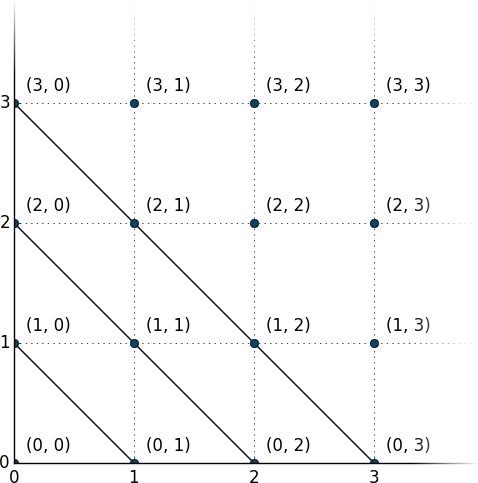
\includegraphics[scale=0.3]{n_croix_n.png}
		\caption{Dénombrabilité de $\mathbb{N}^2$}
		\label{fig-n_croix_n}
	\end{figure}
	
	On obtient la séquence suivante :
	
	\[\begin{array}{l}
		(0,0) \\
		(1,0), (0,1) \\
		(0,2), (1,1), (2,0) \\
		(3,0), (1,2), (2,1), (0,3) \\
		\cdots
	\end{array}.\]
	Plus formellement, l'application qui range les couples de cette manière est 
	\[\begin{array}{cccc}
		\ & \mathbb{N} \times \mathbb{N} & \to & \mathbb{N} \\
		\varphi : & (n,m) & \mapsto & {\underbrace{\frac{(n+m)(n+m+1)}{2}}_{\text{la place du couple dans la ligne}}} +  {\underbrace{\vphantom{\frac{(n+m)(n+m+1)}{2}} m}_{\text{la place du couple dans la ligne}}}
	\end{array}.\]
	
	
	$\varphi$ est bien bijective. $\mathbb{N}^2$ est bien dénombrable.
\end{proof}



De la dénombrabilité de $\mathbb{N}^2$, on peut démontrer le \cref{thm-cartesien}. 

\begin{proof}
	Si $E$ et $F$ sont dénombrables, il existe $\varphi : E \to \mathbb{N}$ et $\psi : F \to \mathbb{N}$ bijectives. On peut alors définir \[ \begin{array}{cccc}
	\ & A \times B & \to & \mathbb{N}^2 \\
	f : & (x,y) & \mapsto & (\varphi(x), \psi(y))
	\end{array}.\]
	
\end{proof}

$f $ est bien bijective. Donc $A \times B$ est bien dénombrable. On procède par récurrence immédiate pour $n$ ensembles. 

On peut maintenant prouver le \cref{thm-union}. 


\begin{proof}
	En effet, on peut écrire $\forall i \in I, A_i = \{x_{n,i}, n \in \mathbb{N}\}$. Chaque élement $x_{n, i}$ est indéxé par sa position $n$ dans $A_i$ et la position $i$ de $(A_i)$ dans $I$. 
	
	Ainsi $A = \bigcup_{i \in I} A_i = \{x_{n, i}, (n,i) \in \mathbb{N} \times I\}$. Les élements $x_{n,i}$ sont indéxés par $\mathbb{N} \times I$ qui est un produit cartésien d'ensembles dénombrables ($I$ est une famille indéxée par $\mathbb{N}$, elle est bien dénombrable). Donc $A$ est dénombrable.
\end{proof}


\section{\texorpdfstring{Dénombrabilité de $\mathbb{Z}$ et de $\mathbb{Q}$}{}}

Intuitivement on pourrait penser que l'ensemble des entiers $\mathbb{Z}$ a une puissance supérieure que $\mathbb{N}$ étant donné qu'il contient deux fois plus d'élements : les entiers naturels et les entiers négatifs. 

\begin{theoremb}{Dénombrabilité de $\mathbb{Z}$}{denz}
	L'ensemble $\mathbb{Z}$ des entiers est dénombrable. 
\end{theoremb}

\begin{proof}
L'idée de la démonstration revient à écrire l'ensemble des entiers, dans l'ordre suivant :  $\mathbb{Z}=\left\lbrace 0,1,(-1),2,(-2),3,(-3) \dots\right\rbrace$ 

	Pour montrer que la puissance de $\mathbb{Z}$ est bien $\aleph_0$, on définit donc l'application $\phi : \mathbb{N} \to \mathbb{Z}$ telle que \[ \forall k \in \mathbb{N}, \left\lbrace \begin{array}{c}
	\phi(2k) = -k \\
	\phi(2k + 1) = k+1
	\end{array} \right. .\]
	
	C'est bien une bijection. Donc $\mathbb{Z}$ est dénombrable. 
\end{proof}

\begin{theoremb}{Dénombrabilité de $\mathbb{Q}$}{denq}
	$\mathbb{Q}$ est dénombrable.
\end{theoremb}

\begin{proof}
	Tout $x \in \mathbb{Q}$ a un unique représentant irréductible $\frac{p}{q}$ où $p \wedge q = 1$. 
	
	Pour établir une bijection entre $\mathbb{Q}$ et $\mathbb{N}$, on commence par écrire un tableau où on range $\frac{p}{q}$ à la colonne $q$ et à la ligne $p$.  
	
	On parcourt le tableau comme c'est indiqué par les flèches dans la \cref{fig-denombQ}. 
	
	On part de $\frac{1}{1}$ dans le tableau. On se déplace à la colonne suivante pour atteindre $\frac{1}{2}$. On parcourt le tableau diagonalement vers le bas pour atteindre $\frac{2}{1}$, on descend d'une case pour obtenir $\frac{3}{1}$ et on parcourt le tableau diagonalement vers le haut jusqu'à atteindre $\frac{1}{3}$, etc. 
	
	On s'aperçoit que chaque nombre rationnel dans le tableau a un et un seul rang $r$ (sa place dans le tableau). L'application $\varphi$ qui range les rationnels $x \in \mathbb{Q}$ dans ce tableau est donc une bijection.
	
	 
\end{proof}
\diagdenomb

A ce stade, on a montré que les ensembles de nombres classiques sont dénombrables, mais bien évidemment, il existe des ensembles non dénombrables, comme $\mathbb{R}$. 


\backmatter
\nocite{*}
\printbibliography
\appendix
\chapter{manuel des commandes}
\begin{theoremb}{Exemple}{exem}
\(\alpha\beta\gamma ABCD=\)
\end{theoremb}
\begin{remarkb}{Remarque}{rema}
\(a\)
\end{remarkb}
\begin{noteb}{Note}{not}
$a$
\end{noteb}
\begin{defb}{Définition}{def}
$a$
\end{defb}
\begin{proof}
\makeatletter
\proofpart{test}
\[TRUC\]
\proofpart{}
\[MACHIN\]
\proofpart*{test}
\[BIDULE\]
\end{proof}
\Cref{thm-exem}, \cref{rem-rema}, \cref{note-not} \cref{def-def} 
\deffunct{f}{E}{F}{x}{f(x)}
\end{document}
